
\documentclass[letterpaper,hide notes,xcolor={table,svgnames},pdftex,10pt]{beamer}
\def\showexamples{t}


%\usepackage[svgnames]{xcolor}

%% Demo talk
%\documentclass[letterpaper,notes=show]{beamer}

\usecolortheme{crane}
\setbeamertemplate{navigation symbols}{}

\usetheme{MyPittsburgh}
%\usetheme{Frankfurt}

%\usepackage{tipa}

\usepackage{hyperref}
\usepackage{graphicx,xspace}
\usepackage[normalem]{ulem}
\usepackage{multicol}
\usepackage{amsmath,amssymb,amsthm,graphicx,xspace}
\newcommand\SF[1]{$\bigstar$\footnote{SF: #1}}

\usepackage[default]{sourcesanspro}
\usepackage[T1]{fontenc}

\newcounter{tmpnumSlide}
\newcounter{tmpnumNote}

% old question code
%\newcommand\question[1]{{$\bigstar$ \small \onlySlide{2}{#1}}}
% \newcommand\nquestion[1]{\ifdefined \presentationonly \textcircled{?} \fi \note{\par{\Large \textbf{?}} #1}}
% \newcommand\nanswer[1]{\note{\par{\Large \textbf{A}} #1}}


 \newcommand\mnote[1]{%
   \addtocounter{tmpnumSlide}{1}
   \ifdefined\showcues {~\tiny\fbox{\arabic{tmpnumSlide}}}\fi
   \note{\setlength{\parskip}{1ex}\addtocounter{tmpnumNote}{1}\textbf{\Large \arabic{tmpnumNote}:} {#1\par}}}

\newcommand\mmnote[1]{\note{\setlength{\parskip}{1ex}#1\par}}

%\newcommand\mnote[2][]{\ifdefined\handoutwithnotes {~\tiny\fbox{#1}}\fi
% \note{\setlength{\parskip}{1ex}\textbf{\Large #1:} #2\par}}

%\newcommand\mnote[2][]{{\tiny\fbox{#1}} \note{\setlength{\parskip}{1ex}\textbf{\Large #1:} #2\par}}

\newcommand\mquestion[2]{{~\color{red}\fbox{?}}\note{\setlength{\parskip}{1ex}\par{\Large \textbf{?}} #1} \note{\setlength{\parskip}{1ex}\par{\Large \textbf{A}} #2\par}\ifdefined \presentationonly \pause \fi}

\newcommand\blackboard[1]{%
\ifdefined   \showblackboard
  {#1}
  \else {\begin{center} \fbox{\colorbox{blue!30}{%
         \begin{minipage}{.95\linewidth}%
           \hspace{\stretch{1}} Some space intentionally left blank; done at the blackboard.%
         \end{minipage}}}\end{center}}%
         \fi%
}



%\newcommand\q{\tikz \node[thick,color=black,shape=circle]{?};}
%\newcommand\q{\ifdefined \presentationonly \textcircled{?} \fi}

\usepackage{listings}
\lstset{%
  keywordstyle=\bfseries,
  aboveskip=15pt,
  belowskip=15pt,
  captionpos=b,
  identifierstyle=\ttfamily,
  escapeinside={(*@}{@*)},
  stringstyle=\ttfamiliy,
  frame=lines,
  numbers=left, basicstyle=\scriptsize, numberstyle=\tiny, stepnumber=0, numbersep=2pt}

\usepackage{siunitx}
\newcommand\sius[1]{\num[group-separator = {,}]{#1}\si{\micro\second}}
\newcommand\sims[1]{\num[group-separator = {,}]{#1}\si{\milli\second}}
\newcommand\sins[1]{\num[group-separator = {,}]{#1}\si{\nano\second}}
\sisetup{group-separator = {,}, group-digits = true}

%% -------------------- tikz --------------------
\usepackage{tikz}
\usetikzlibrary{positioning}
\usetikzlibrary{arrows,backgrounds,automata,decorations.shapes,decorations.pathmorphing,decorations.markings,decorations.text}

\tikzstyle{place}=[circle,draw=blue!50,fill=blue!20,thick, inner sep=0pt,minimum size=6mm]
\tikzstyle{transition}=[rectangle,draw=black!50,fill=black!20,thick, inner sep=0pt,minimum size=4mm]

\tikzstyle{block}=[rectangle,draw=black, thick, inner sep=5pt]
\tikzstyle{bullet}=[circle,draw=black, fill=black, thin, inner sep=2pt]

\tikzstyle{pre}=[<-,shorten <=1pt,>=stealth',semithick]
\tikzstyle{post}=[->,shorten >=1pt,>=stealth',semithick]
\tikzstyle{bi}=[<->,shorten >=1pt,shorten <=1pt, >=stealth',semithick]

\tikzstyle{mut}=[-,>=stealth',semithick]

\tikzstyle{treereset}=[dashed,->, shorten >=1pt,>=stealth',thin]

\usepackage{ifmtarg}
\usepackage{xifthen}
\makeatletter
% new counter to now which frame it is within the sequence
\newcounter{multiframecounter}
% initialize buffer for previously used frame title
\gdef\lastframetitle{\textit{undefined}}
% new environment for a multi-frame
\newenvironment{multiframe}[1][]{%
\ifthenelse{\isempty{#1}}{%
% if no frame title was set via optional parameter,
% only increase sequence counter by 1
\addtocounter{multiframecounter}{1}%
}{%
% new frame title has been provided, thus
% reset sequence counter to 1 and buffer frame title for later use
\setcounter{multiframecounter}{1}%
\gdef\lastframetitle{#1}%
}%
% start conventional frame environment and
% automatically set frame title followed by sequence counter
\begin{frame}%
\frametitle{\lastframetitle~{\normalfont(\arabic{multiframecounter})}}%
}{%
\end{frame}%
}
\makeatother

\makeatletter
\newdimen\tu@tmpa%
\newdimen\ydiffl%
\newdimen\xdiffl%
\newcommand\ydiff[2]{%
    \coordinate (tmpnamea) at (#1);%
    \coordinate (tmpnameb) at (#2);%
    \pgfextracty{\tu@tmpa}{\pgfpointanchor{tmpnamea}{center}}%
    \pgfextracty{\ydiffl}{\pgfpointanchor{tmpnameb}{center}}%
    \advance\ydiffl by -\tu@tmpa%
}
\newcommand\xdiff[2]{%
    \coordinate (tmpnamea) at (#1);%
    \coordinate (tmpnameb) at (#2);%
    \pgfextractx{\tu@tmpa}{\pgfpointanchor{tmpnamea}{center}}%
    \pgfextractx{\xdiffl}{\pgfpointanchor{tmpnameb}{center}}%
    \advance\xdiffl by -\tu@tmpa%
}
\makeatother
\newcommand{\copyrightbox}[3][r]{%
\begin{tikzpicture}%
\node[inner sep=0pt,minimum size=2em](ciimage){#2};
\usefont{OT1}{phv}{n}{n}\fontsize{4}{4}\selectfont
\ydiff{ciimage.south}{ciimage.north}
\xdiff{ciimage.west}{ciimage.east}
\ifthenelse{\equal{#1}{r}}{%
\node[inner sep=0pt,right=1ex of ciimage.south east,anchor=north west,rotate=90]%
{\raggedleft\color{black!50}\parbox{\the\ydiffl}{\raggedright{}#3}};%
}{%
\ifthenelse{\equal{#1}{l}}{%
\node[inner sep=0pt,right=1ex of ciimage.south west,anchor=south west,rotate=90]%
{\raggedleft\color{black!50}\parbox{\the\ydiffl}{\raggedright{}#3}};%
}{%
\node[inner sep=0pt,below=1ex of ciimage.south west,anchor=north west]%
{\raggedleft\color{black!50}\parbox{\the\xdiffl}{\raggedright{}#3}};%
}
}
\end{tikzpicture}
}


%% --------------------

%\usepackage[excludeor]{everyhook}
%\PushPreHook{par}{\setbox0=\lastbox\llap{MUH}}\box0}

%\vspace*{\stretch{1}

%\setbox0=\lastbox \llap{\textbullet\enskip}\box0}

\setlength{\parskip}{\fill}

\newcommand\noskips{\setlength{\parskip}{1ex}}
\newcommand\doskips{\setlength{\parskip}{\fill}}

\newcommand\xx{\par\vspace*{\stretch{1}}\par}
\newcommand\xxs{\par\vspace*{2ex}\par}
\newcommand\tuple[1]{\langle #1 \rangle}
\newcommand\code[1]{{\sf \footnotesize #1}}
\newcommand\ex[1]{\uline{Example:} \ifdefined \presentationonly \pause \fi
  \ifdefined\showexamples#1\xspace\else{\uline{\hspace*{2cm}}}\fi}

\newcommand\ceil[1]{\lceil #1 \rceil}


\AtBeginSection[]
{
   \begin{frame}
       \frametitle{Outline}
       \tableofcontents[currentsection]
   \end{frame}
}



\pgfdeclarelayer{edgelayer}
\pgfdeclarelayer{nodelayer}
\pgfsetlayers{edgelayer,nodelayer,main}

\tikzstyle{none}=[inner sep=0pt]
\tikzstyle{rn}=[circle,fill=Red,draw=Black,line width=0.8 pt]
\tikzstyle{gn}=[circle,fill=Lime,draw=Black,line width=0.8 pt]
\tikzstyle{yn}=[circle,fill=Yellow,draw=Black,line width=0.8 pt]
\tikzstyle{empty}=[circle,fill=White,draw=Black]
\tikzstyle{bw} = [rectangle, draw, fill=blue!20, 
    text width=4em, text centered, rounded corners, minimum height=2em]
    
    \newcommand{\CcNote}[1]{% longname
	This work is licensed under the \textit{Creative Commons #1 3.0 License}.%
}
\newcommand{\CcImageBy}[1]{%
	\includegraphics[scale=#1]{creative_commons/cc_by_30.pdf}%
}
\newcommand{\CcImageSa}[1]{%
	\includegraphics[scale=#1]{creative_commons/cc_sa_30.pdf}%
}
\newcommand{\CcImageNc}[1]{%
	\includegraphics[scale=#1]{creative_commons/cc_nc_30.pdf}%
}
\newcommand{\CcGroupBySa}[2]{% zoom, gap
	\CcImageBy{#1}\hspace*{#2}\CcImageNc{#1}\hspace*{#2}\CcImageSa{#1}%
}
\newcommand{\CcLongnameByNcSa}{Attribution-NonCommercial-ShareAlike}

\newenvironment{changemargin}[1]{% 
  \begin{list}{}{% 
    \setlength{\topsep}{0pt}% 
    \setlength{\leftmargin}{#1}% 
    \setlength{\rightmargin}{1em}
    \setlength{\listparindent}{\parindent}% 
    \setlength{\itemindent}{\parindent}% 
    \setlength{\parsep}{\parskip}% 
  }% 
  \item[]}{\end{list}} 




\title{Lecture  11 --- Decomposition: Functional-Dependency Theory }

\author{Jeff Zarnett \\ \small \texttt{jzarnett@uwaterloo.ca}}
\institute{Department of Electrical and Computer Engineering \\
  University of Waterloo}
\date{\today}


\begin{document}

\begin{frame}
  \titlepage

 \end{frame}



\begin{frame}
\frametitle{Seeking Closure}

Earlier we talked about the closure of a set of functional dependencies. 

Recall from earlier that the closure contains all the functional dependencies that are explicitly satisfied as well as those that are logically implied. 

That is, if $A \rightarrow B$ and $B \rightarrow C$ then it is implied that $A \rightarrow C$.

\end{frame}



\begin{frame}
\frametitle{Seeking Closure}
If the functional dependencies are $A \rightarrow B$ and $B \rightarrow C$ then we know that for two tuples $t_{1}$ and $t_{2}$ if $t_{1}[A] = t_{2}[A]$ then $t_{1}[B] = t_{2}[B]$ and $t_{1}[C] = t_{2}[C]$. 

The notation to show the closure of a set $F$ of functional dependencies is $F^{+}$ as previously discussed.

\end{frame}


\begin{frame}
\frametitle{Computing Closure}

If $F$ is large there are many rules and many implied rules and we have to construct every logically implied element of $F^{+}$ from first principles. 

Instead, we would like to use \textit{axioms}, handy rules of inference, that allow us to reason about the dependencies in a simpler way. 


\end{frame}


\begin{frame}
\frametitle{Armstrong's Axioms}
The first three axions are simple enough and are called \alert{Armstrong's Axioms}:

\begin{itemize}
	\item \textbf{Reflexivity}: If $\alpha$ is a set of attributes and $\beta$ is contained within $\alpha$, then $\alpha \rightarrow \beta$ holds.
	\item \textbf{Augmentation}: If $\alpha \rightarrow \beta$ holds and $\gamma$ is a set of attributes, then $\gamma\alpha \rightarrow \gamma\beta$ holds.
	\item \textbf{Transitivity}: If $\alpha \rightarrow \beta$ holds and $\beta \rightarrow \gamma$ holds, then $\alpha \rightarrow \gamma$ holds.
\end{itemize}

\end{frame}



\begin{frame}
\frametitle{Derived Rules (Shortcuts)}

Some convenient shortcuts:

\begin{itemize}
	\item \textbf{Union}: If $\alpha \rightarrow \beta$ holds and $\alpha \rightarrow \gamma$ holds, then $\alpha \rightarrow \beta\gamma$ holds.
	\item \textbf{Decomposition}: If $\alpha \rightarrow \beta\gamma$ holds, then  $\alpha \rightarrow \beta$ holds and $\alpha \rightarrow \gamma$ holds (reverse of previous rule).
	\item \textbf{Pseudotransitivity}: If $\alpha \rightarrow \beta$ holds and $\gamma\beta \rightarrow \delta$ holds, then $\alpha\gamma \rightarrow \delta$ holds.
\end{itemize}

\end{frame}


\begin{frame}
\frametitle{Functional Dependency Theory Example}

The relation $r$ has the attributes $(A, B, C, G, H, I)$.

The functional dependencies are: (1) $A \rightarrow B$, (2) $A \rightarrow C$, (3) $CG \rightarrow H$, (4) $CG \rightarrow I$, (5) $B \rightarrow H$.

Based on the rules that we have, what logically implied functional dependencies can we observe?

\end{frame}



\begin{frame}
\frametitle{Functional Dependency Theory Example}

There are five:
\begin{itemize}
	\item $A \rightarrow H$ which is found by transitivity ($A \rightarrow B$ and $B \rightarrow H$).
	\item $A \rightarrow BC$ which is found by the union rule ($A \rightarrow B$ and $A \rightarrow C$).
	\item $A \rightarrow BCH$ which is found by the union rule ($A \rightarrow BC$ and $A \rightarrow H$).
	\item $CG \rightarrow HI$ which is found by the union rule ($CG \rightarrow H$ and $CG \rightarrow I$).
	\item $AG \rightarrow I$ which is found by pseudotransitivity ($A \rightarrow C$ and $CG \rightarrow I$).
\end{itemize}


\end{frame}



\begin{frame}
\frametitle{Computing the Closure}

\begin{enumerate}
	\item The initial condition is that $F^{+}$ begins as $F$.
	\item For each functional dependency $f$ in F+ $F^{+}$:
	\begin{enumerate}
		\item apply the transitivity rule to $f$ and add it to $F^{+}$
		\item apply the augmentation rule to $f$ and add it to $F^{+}$
	\end{enumerate}
	\item For each pair of functional dependencies $f_{1}$ and $f_{2}$, if they can be combined using transitivity, add the newly created combination to $F^{+}$.
	\item If anything was added in steps 2 or 3, go back to step 2; otherwise the algorithm terminates.
\end{enumerate}

\end{frame}



\begin{frame}
\frametitle{Closure of Attribute Sets}

Suppose we have some attribute(s) $\alpha$ and we wish to determine if it is a superkey. 

The strategy we will use requires us to compute the set of attributes that are \alert{functionally determined} by $\alpha$. 

An attribute $B$ is functionally determined by $\alpha$ if $\alpha \rightarrow B$. 

Then the simple algorithm requires us to compute $F^{+}$...

\end{frame}



\begin{frame}
\frametitle{More Efficient Algorithm}

A more efficient algorithm:

\begin{enumerate}
	\item The initial condition is that $\alpha^{+}$ begins as $\alpha$.
	\item For each functional dependency $\beta \rightarrow \gamma$ in $F$,
		if $\beta$ is contained in $\alpha^{+}$, then $\gamma$ is added to $\alpha^{+}$
	\item If anything was added in step 2, repeat step 2; if nothing was added, the algorithm terminates.
\end{enumerate}

Much like computing the closure of $F$, here we compute the closure of $\alpha$. 

\end{frame}



\begin{frame}
\frametitle{Back to the Example}

Given the rules, is $A$ a superkey? Let's go through the steps. 

The initial condition is that $A$ is in $\alpha^{+}$ (the result). 

\end{frame}



\begin{frame}
\frametitle{Back to the Example}

The result is $ABCH$. 

This is not the full set ($ABCGHI$) and therefore we conclude that $A$ is not a superkey.

\end{frame}



\begin{frame}
\frametitle{Back to the Example}

This procedure can be repeated for any individual attribute and we will quickly find that no single attribute is a superkey for this relation. 

This is perhaps somewhat obvious from our list of functional dependencies. 

If we look carefully at them we can notice that neither $A$ nor $G$ ever appears on the right hand side of any of the functional dependencies.

All the other attributes do.


\end{frame}



\begin{frame}
\frametitle{Back to the Example}

That gives us a hint that a superkey might be $AG$, and that assumption can of course be tested by following the rules as above.

If our candidate is $AG$ as suggested, we start off by saying the result is $AG$. 

We will, in fact, find that $AG$ is a superkey.

\end{frame}




\begin{frame}
\frametitle{Use of Attribute Closure}

There are three ways we can use this attribute closure algorithm:
\begin{itemize}
	\item As above, to test if $\alpha$ is a superkey.
	\item Check if a functional dependency holds (by determining if it is in $\alpha^{+}$.
	\item As another way to compute $F^{+}$; we just compute the $\alpha^{+}$ for each $\alpha$ and then combine them. 
\end{itemize}

\end{frame}



\begin{frame}
\frametitle{Canonical Cover}

Suppose we have a set of functional dependencies $F$ on a relation. 

Whenever a user wants to update the data inside this relation, the database system must check that all functional dependencies in $F$ are still satisfied. 

\end{frame}



\begin{frame}
\frametitle{Canonical Cover}

We would like to simplify the set to a minimal number of rules that has the same closure.

For example, if the rules say $A \rightarrow B$ and $B \rightarrow C$ and $A \rightarrow C$ we can immediately identify that there is redundancy. 

We could remove the rule $A \rightarrow C$.

You could argue that this sort of thing should not be necessary: designers should not introduce redundant rules and if they do it is their own fault...

\end{frame}



\begin{frame}
\frametitle{Extraneous Dependencies}

Formally speaking, an attribute of a functional dependency is \alert{extraneous} (unnecessary) under the following two scenarios:
\begin{itemize}
	\item $A$ is extraneous in $\alpha$ if $A$ is in $\alpha$ and $F$ logically implies $(F - (\alpha \rightarrow \beta)) \cup ((\alpha - A) \rightarrow \beta))$.
	\item $A$ is extraneous in $\beta$ if $A$ is in $\beta$ and the set of functional dependencies $(F - (\alpha \rightarrow \beta)) \cup (\alpha \rightarrow (\beta - A))$ logically implies $F$.
\end{itemize}

\end{frame}



\begin{frame}
\frametitle{Extraneous Dependencies}
To check if $A$ is extraneous on the right hand side, the routine is fairly simple.

Remove $A$ from the right hand side ($\beta$) from the rule that it is in (e.g., if the rule is $D \rightarrow AB$, replace it with $D \rightarrow B$).

Then compute the canonical cover of $\alpha$ (in this example, $D$). If the canonical cover included $A$, then $A$ was extraneous in $\beta$.

\end{frame}



\begin{frame}
\frametitle{Extraneous Dependencies}

To check if $A$ is extraneous on the left hand side: 

Remove $A$ from the left hand side ($\alpha$) and check if this reduced set still functionally determines $\beta$. 

So if the rule is $DF \rightarrow GH$, remove $F$ and we are left with the uncertain rule $D \rightarrow GH$, which we need to test to be sure. 

We compute the closure of $D$ without this modified rule and see if it includes $GH$. 

If it does, then $F$ was extraneous in the left hand side.

\end{frame}


\begin{frame}
\frametitle{Canonical Cover}

The canonical cover for $F$ is denoted $F_{c}$ and it is a minimal representation of $F$. 

It requires two rules: (1) no functional dependency in $F_{c}$ has an extraneous attribute, and (2) the left side of each functional dependency is unique. 


\end{frame}



\begin{frame}
\frametitle{Canonical Cover Example}

The schema is simple $(A, B, C)$ and our functional dependencies are ($A \rightarrow BC, B \rightarrow C, A \rightarrow B, AB \rightarrow C$). 

Well, anyway, it is simple enough, we can use the union rule to combine the rule $A \rightarrow BC$ and $A \rightarrow B$ (pretty obvious). 

And then we can remove extraneous attributes to get this down to $A \rightarrow B$ and $B \rightarrow C$. 

This is slightly redundant and we can figure out by transitivity that $A \rightarrow BC$. 

\end{frame}



\begin{frame}
\frametitle{Canonical Cover Example 2}

Another example:  our schema has more attributes and the functional dependencies are ($B \rightarrow A, D \rightarrow A, AB \rightarrow D$). 

In this case, all the left hand sides are different, so we can't combine any that way. 

The right hand sides are all single attributes so we don't need to look for extraneous attributes there. 

But we should look at the left hand side. 

\end{frame}



\begin{frame}
\frametitle{Canonical Cover Example 2}

The only one that is not minimal there is the functional dependency $AB \rightarrow D$ and we would like to know if we can eliminate $A$ or $B$ from the left side.

Looking at the rule that says $B \rightarrow A$ we can probably reason pretty well that if $B \rightarrow A$ then $B \rightarrow AB$.

So we can replace the one double-left-side rule with $B \rightarrow D$. 

Then we have a set that is equivalent: ($B \rightarrow A, D \rightarrow A, B \rightarrow D$). 

There is some redundancy here, though, and we could find out that $B \rightarrow A$ can be eliminated, leaving us with ($B \rightarrow D, D \rightarrow A$).

\end{frame}



\begin{frame}
\frametitle{Multiple Correct Answers}

Because canonical cover is about finding a minimal equivalent set, it is not necessarily that there is only one correct answer. 

If there is redundancy, we may need to delete one of two attributes (but not both). 

Let's go back to the example from earlier with the three attributes. Our functional dependencies are still ($A \rightarrow BC, B \rightarrow C, A \rightarrow B, AB \rightarrow C$). 

If we test $A \rightarrow BC$ we will find that both $B$ and $C$ are extraneous. 

One person might choose to delete $B$ and another person might choose to delete $C$. Neither choice is wrong.

\end{frame}



\begin{frame}
\frametitle{Lossless Decomposition}

Decomposition is breaking up a relation into two or more smaller ones. 

The motivations for doing so are something we will come back to later on, but for the moment, just assume there are good reasons. 

A decomposition is \alert{lossless} if no information is lost by splitting a relation $r$ into smaller relations $r_{1}$ and $r_{2}$. 

If information is loss it is called \alert{lossy} (and that is undesirable).

$\Pi_{R_{1}}(r) \bowtie \Pi_{R_{2}}(r) = r$

\end{frame}



\begin{frame}
\frametitle{Lossless Decomposition}

If the decomposition is lossless then every functional dependency $f$ in $F$ holds in spite of the fact that the relation is split. 

But we can't really cheat and just ``forget'' to put in the functional dependencies to make it work, now can we?

There needs to be some attribute or attributes that link together the two tables.

One relation needs to have some way of referencing another.

\end{frame}



\begin{frame}
\frametitle{Lossless Decomposition}

The formal definition for a lossless decomposition says that one of the following must hold on the two relations: 

$R_{1} \cap R_{2} \rightarrow R_{1}$ or  $R_{1} \cap R_{2} \rightarrow R_{2}$. 

That is to say, the intersection of the two relations most be sufficient to uniquely identify one of the two of them. 

\end{frame}



\begin{frame}
\frametitle{Lossless Decomposition Example}

Suppose we have employee with \textit{id, name, street, city, province, postalcode}.

We tried to split it into $r_{1}$ as \textit{id, name}, and $r_{2}$ as \textit{name, street, city, province, postcode}. 

Is this going to work? The intersection of these two is \textit{name} and this is not a superkey for either $r_{1}$ or $r_{2}$ because names are not unique.

\end{frame}



\begin{frame}
\frametitle{Testing Lossless Decomposition}

There is a formal way for testing that dependencies have been preserved. 

There is a computationally expensive algorithm outlined in the textbook. 

There's also one that is premised on the idea that if each functional dependency $f$ can be tested on one relation only, then just test it on that relation. 

Unfortunately that last assumption is not necessarily true; it could happen that a functional dependency is across tables...

\end{frame}


\begin{frame}
\frametitle{Lossless Decomposition Algorithm}

Our solution is then a modified algorithm that does not require us to compute the closure of $F$. 

The algorithm is executed for each functional dependency $\alpha \rightarrow \beta$:


\begin{enumerate}
	\item $result$ = $\alpha$
	\item for reach relation $R_{i}$ in the decomposition
	\begin{enumerate}
		\item $result = result \cup (  (result \cap R_{i})^{+} \cap R_{i} )$
	    \item if $result$ did not change at all, break out of the for loop
	    \end{enumerate}
\end{enumerate}

If $result$ contains all attributes in $\beta$, then the dependency is preserved. And this must hold for all dependencies $\alpha \rightarrow \beta$.

\end{frame}



\begin{frame}
\frametitle{Decomposition Algorithms: BCNF}
The initial state is the relations that we have, and we also need to then compute $F^{+}$. Then the steps are:

\begin{center}
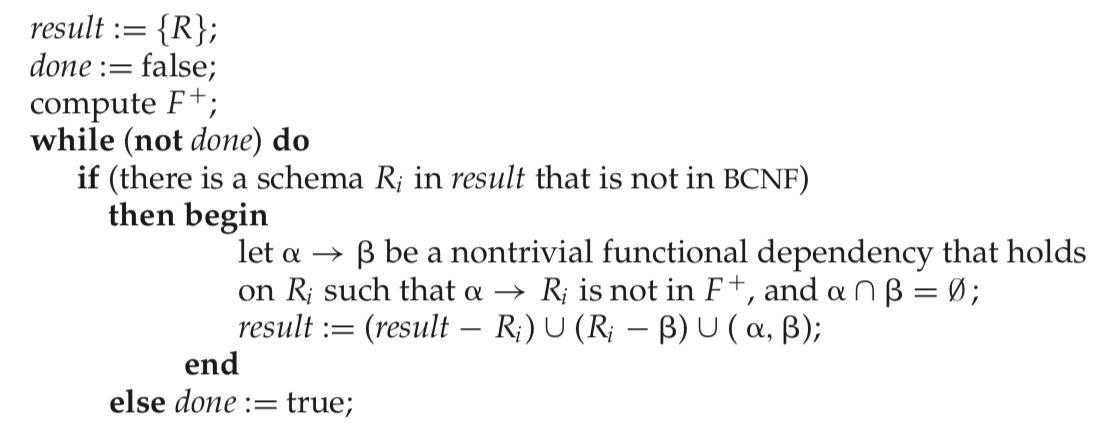
\includegraphics[width=0.7 \textwidth]{images/bcnf-algorithm}
\end{center}

The algorithm produces relations in BCNF and a lossless decomposition. 

This is because when we replace a schema $R_{i}$ with $(R_{i} - \beta)$ and $(\alpha, \beta)$ then the intersection of these two relations is $\alpha$.

\end{frame}



\begin{frame}
\frametitle{Decomposition Algorithms: 3NF}


\begin{center}
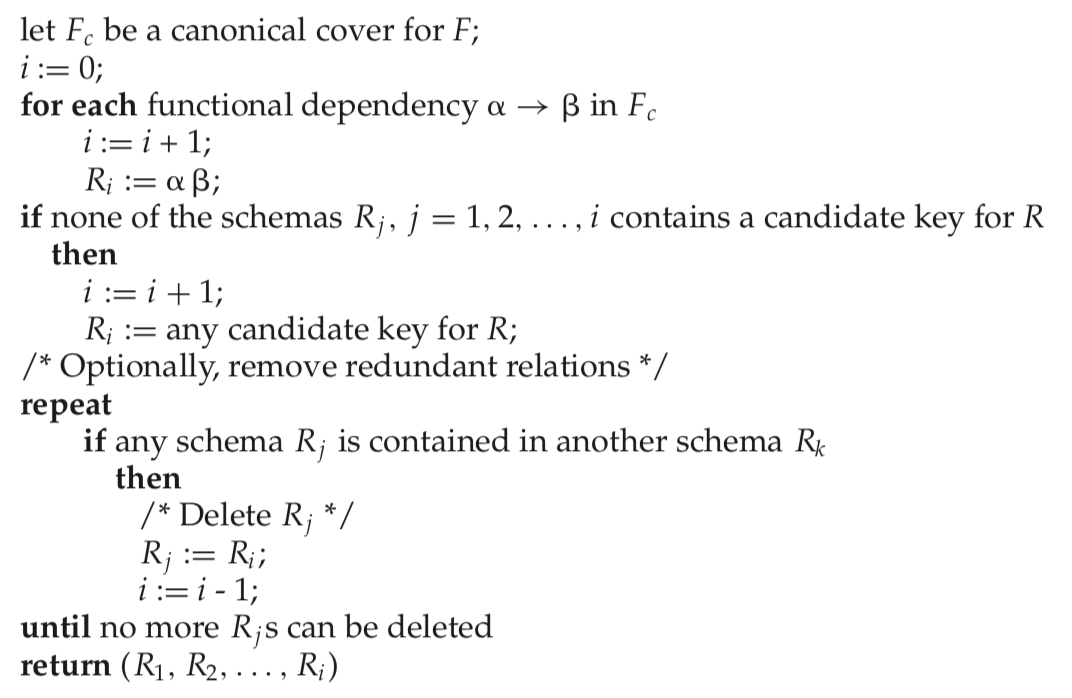
\includegraphics[width=0.7\textwidth]{images/3nf-algorithm}
\end{center}



\end{frame}



\end{document}

